
\section{Results and Analysis}



% \label{sec:main_results}
% Table~\todo{Table X} compares Omni (No-RAG) and RAG-InfiniSST under matched SimulEval settings.
% We report BLEU, StreamLAAL, StreamLAAL\_CA, and \textsc{TermAcc}.
% \todo{Add Table X placeholder.}

\subsection{Main Results}

\paragraph{\method substantially improves terminology accuracy}
Figure~\ref{fig:main_result_1} shows that \method outperforms InfiniSST in exact-match terminology accuracy across all 12 ACL language--latency settings, with gains of 12.3--21.4 percentage points. Figure~\ref{fig:eso_de_main} presents the English--German results on ESO, where \method yields larger gains of 26.0--31.2 points across the four latency settings. We attribute the larger gains on ESO to the difficulty of recognizing and translating specialized oncology terms. By contrast, many terms annotated in ACL 60/60 are common words, such as \emph{words}, \emph{model}, and \emph{weights}, which are comparatively easy to translate. Notably, \method also surpasses the Offline baseline, demonstrating that access to the complete speech context alone is insufficient for reliable terminology translation. Although a gap to Offline + GT Terms remains because retrieval is imperfect, it is typically below five percentage points, indicating that \method captures most of the benefit of oracle terminology access. The form-aware evaluation in Appendix~\ref{app:form_aware_metric} confirms that these conclusions are not artifacts of orthographic or inflectional variation.

\paragraph{RASST improves overall translation quality}
On ACL 60/60, \method achieves higher BLEU than InfiniSST in 10 of the 12 settings, with a maximum gain of 3 BLEU points. By contrast, the two systems obtain comparable COMET scores. One likely explanation is that \method inserts retrieved target terms verbatim, which is more favored by a surface-form metric such as BLEU than by a neural semantic metric such as COMET. Moreover, although aligned target terms occur in 83.76--86.54\% of ACL sentences, they constitute only 10.66--18.06\% of the target tokens. Improvements in terminology accuracy therefore affect a limited proportion of the corpus.

\paragraph{\method is robust to large glossary size}
Figure~\ref{fig:ablation_glossary_bank} shows that \method remains competitive as the glossary scales to 10K terms. Going from 0.2K to 1K and then 10K terms gradually reduces terminology accuracy by less than 2\% and BLEU by less than 1 point, and \method still clearly outperforms the no-retrieval baseline.


\begin{table}[t]
\centering
\small
\begin{tabular}{lcccc}
\toprule
\textbf{Chunk Size (s)} & 0.96 & 1.92 & 2.88 & 3.84 \\
\midrule
Wall-Clock Time (s)    & 0.036 & 0.042 & 0.042 & 0.043 \\
\bottomrule
\end{tabular}
\caption{Retriever computation cost across speech chunk sizes. The retriever's overhead is negligible.}
\label{tab:rag_compute_rtf}
\vspace{-0.5cm}
\end{table}

\paragraph{\method is computationally efficient}
Table~\ref{tab:rag_compute_rtf} reports the additional computational cost introduced by the retriever. We run evaluation on two NVIDIA RTX A6000 GPUs, serving the Speech LLM with vLLM at tensor parallelism 2 and \texttt{gpu\_memory\_utilization}{=}0.72, while the retriever encoder fits in the remaining GPU memory. The retriever's wall-clock time per chunk is at most $3.75\%$ of the chunk size, and becomes smaller as the chunk grows, which makes it negligible in practice.

\subsection{Ablation Studies}
\label{sec:ablations}

\paragraph{Retriever hard negatives and threshold}
We examine the effect of training-time hard negatives and the inference-time threshold $\tau$. In addition to the default retriever trained with $N{=}1024$ hard negatives, we train two variants with $N{=}256$ and $N{=}0$. We evaluate their precision and recall on the GigaSpeech dev set against three glossaries: a 1K glossary built from GigaSpeech noun phrases, and 10K and 100K extensions with Wikidata terms unseen during training. For each (retriever variant, glossary) pair, we sweep $\tau$ from $0$ to $1$ to obtain a precision-recall curve. 

Figure~\ref{fig:ablation_hn_tau} shows the results. First, increasing $N$ yields clearly higher recall at the same precision, confirming the value of hard-negative mining. Second, recall degrades as the glossary grows. Based on these curves, we set $\tau{=}0.78$ at inference: it costs at most a 1\% drop in recall while roughly reducing the retrieval noise by half. Compared with $\tau=0$ in Figure \ref{fig:ablation_speechllm_tau}, $\tau=0.78$ achieves higher terminology accuracy. 

\paragraph{Multi-Scale Inference}
We examine the contribution of multi-scale inference. As described in Section~\ref{sec:retriever}, \method's retriever queries with speech windows at multiple scales and keeps the terms with the highest similarities. We compare against two variants. The first reuses our retriever but queries with only the largest window at inference time, but this introduces a training–inference mismatch, since the retriever was trained with MFA-aligned windows around each term. The second variant removes this mismatch by training the retriever directly with the largest window, without MFA-based window localization. Results are shown in Figure \ref{fig:ablation_multiscale}. Multi-scale inference combined with MFA-localized training performs best: it loses less than 1\% in recall when scaling from 1K to 100K glossary, compared to drops of over 2\% and 5\% for the two variants. The end-to-end En--Zh evaluation at latency multiplier 2 in Table~\ref{tab:multiscale_e2e} confirms that this retrieval gain reaches the translation output: multi-scale inference achieves 90.00\% terminology accuracy, versus 84.72\% for largest-window inference and 73.93\% when the retriever is also trained on the largest window.

\begin{figure}[t]
    \centering
    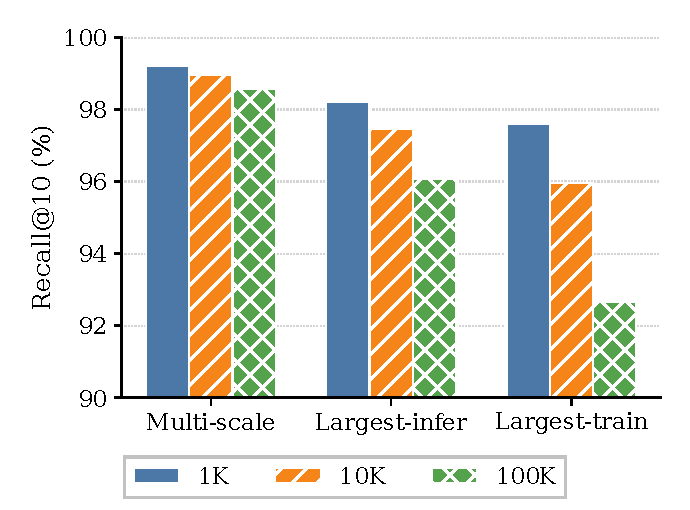
\includegraphics[width=\linewidth]{latex/figures/multiscale_inference_ablation_devraw.pdf}
    \caption{Recall@10 on the GigaSpeech dev set for multi-scale inference in \method and two variants. Largest-infer uses the same retriever as \method but queries with only the largest window at inference. Largest-train trains the retriever with the largest window instead of the MFA-localized window. Multi-scale inference combined with MFA-localized training performs best.}
    \label{fig:ablation_multiscale}
\end{figure}

\begin{table}[t]
\centering
% \color{red}
\small
\setlength{\tabcolsep}{3.5pt}
\begin{tabular}{lrrr}
\toprule
Variant & BLEU $\uparrow$ & LAAL (ms) $\downarrow$ & TERM\_ACC $\uparrow$ \\
\midrule
Multi-scale & \textbf{47.8780} & \textbf{1814.34} & \textbf{90.00} \\
Largest-infer & 47.8261 & 1868.37 & 84.72 \\
Largest-train & 45.7960 & 1863.20 & 73.93 \\
\bottomrule
\end{tabular}
\caption{End-to-end ablation of retrieval strategies on ACL En--Zh at latency multiplier 2.}
\label{tab:multiscale_e2e}
\end{table}

\begin{figure*}
    \centering
    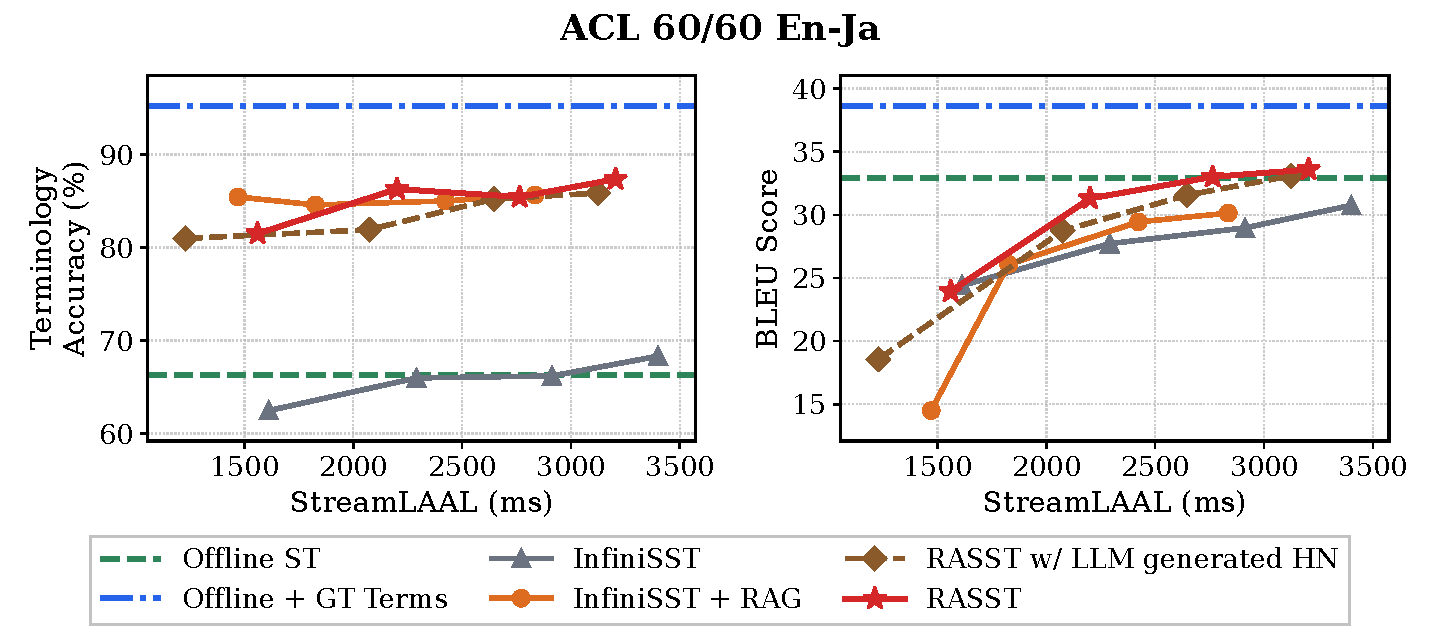
\includegraphics[width=0.9\linewidth]{latex/figures/speechllm_ablation_ja.pdf}
    \caption{Quality–latency trade-off of \method against two training-data variants: a version trained with LLM-generated distractors, and \textit{InfiniSST + RAG}, which adds retrieval at inference to a model not trained with terms $G_i$. \method achieves the best overall trade-off.}
    \label{fig:ablation_speechllm}
\end{figure*}


\paragraph{Speech LLM Training Data}
We ablate the distractor-sampling strategy used to construct $G_i$ during Speech LLM training. Besides retriever mined distractors in \method, we train two variants: one with LLM-generated distractors, and one with no retrieved terms at all (equivalent to InfiniSST). At inference, all variants use the same retriever to populate $G_i$ from the speech chunk before the Speech LLM generates the translation. Results are shown in Figure \ref{fig:ablation_speechllm}. The model trained with LLM-generated distractors achieves slightly lower terminology accuracy and BLEU than \method. More surprisingly, \textit{InfiniSST + RAG}, which sees no retrieved terms during training but is given them at inference, matches \method's terminology accuracy but has much worse BLEU score. Inspecting its outputs, we find that it tends to copy retrieved terms verbatim without checking whether they actually appear in the source or inserting them at the right time.

More ablations on retriever training data, encoder choice, context length, and tag supervision can be found in Appendix \ref{sec:apdx_ablation}.

\subsection{Robustness Analysis}

We evaluate the robustness of \method to variations in glossary and retrieval quality in Appendix~\ref{sec:robustness_analysis}.

\subsection{Qualitative Analysis}

We additionally present a case study examining the behavior of \method in Appendix~\ref{sec:qualitative_analysis}.

